\documentclass[a4paper,12pt]{article}
% ============================================================
% Общий преамбул для отчётов по лабораторным работам (labs_lpr)
% Подключается из report/main.tex командой:
%   % ============================================================
% Общий преамбул для отчётов по лабораторным работам (labs_lpr)
% Подключается из report/main.tex командой:
%   % ============================================================
% Общий преамбул для отчётов по лабораторным работам (labs_lpr)
% Подключается из report/main.tex командой:
%   \input{../../common/latex_template/preamble.tex}
% ============================================================

% Поддержка русского языка и кодировки
\usepackage[T2A]{fontenc}
\usepackage{lmodern}
\usepackage[utf8]{inputenc}
\usepackage[russian]{babel}

% Математические пакеты
\usepackage{amsmath, amssymb}

% Настройка полей
\usepackage{geometry}
\geometry{top=2cm, bottom=2cm, left=2.5cm, right=1.5cm}

% Колонтитулы
\usepackage{fancyhdr}
\usepackage{graphicx}

% Современные таблицы
\usepackage{tabularray}

% Работа с csv файлами
\usepackage{csvsimple-l3}
\usepackage{tikz}

% Графики
\usepackage{pgfplots}
\pgfplotsset{compat=1.18}

% Ссылки
% \usepackage{hyperref} % гипперссылки, нужно оформление вместо красного квадрата
\usepackage[russian]{cleveref} % умные ссылки, нужно переоформление для формул, рисунков и тд (вместо ф-л что-то нужно придумать)

% ============================================================

% Поддержка русского языка и кодировки
\usepackage[T2A]{fontenc}
\usepackage{lmodern}
\usepackage[utf8]{inputenc}
\usepackage[russian]{babel}

% Математические пакеты
\usepackage{amsmath, amssymb}

% Настройка полей
\usepackage{geometry}
\geometry{top=2cm, bottom=2cm, left=2.5cm, right=1.5cm}

% Колонтитулы
\usepackage{fancyhdr}
\usepackage{graphicx}

% Современные таблицы
\usepackage{tabularray}

% Работа с csv файлами
\usepackage{csvsimple-l3}
\usepackage{tikz}

% Графики
\usepackage{pgfplots}
\pgfplotsset{compat=1.18}

% Ссылки
% \usepackage{hyperref} % гипперссылки, нужно оформление вместо красного квадрата
\usepackage[russian]{cleveref} % умные ссылки, нужно переоформление для формул, рисунков и тд (вместо ф-л что-то нужно придумать)

% ============================================================

% Поддержка русского языка и кодировки
\usepackage[T2A]{fontenc}
\usepackage{lmodern}
\usepackage[utf8]{inputenc}
\usepackage[russian]{babel}

% Математические пакеты
\usepackage{amsmath, amssymb}

% Настройка полей
\usepackage{geometry}
\geometry{top=2cm, bottom=2cm, left=2.5cm, right=1.5cm}

% Колонтитулы
\usepackage{fancyhdr}
\usepackage{graphicx}

% Современные таблицы
\usepackage{tabularray}

% Работа с csv файлами
\usepackage{csvsimple-l3}
\usepackage{tikz}

% Графики
\usepackage{pgfplots}
\pgfplotsset{compat=1.18}

% Ссылки
% \usepackage{hyperref} % гипперссылки, нужно оформление вместо красного квадрата
\usepackage[russian]{cleveref} % умные ссылки, нужно переоформление для формул, рисунков и тд (вместо ф-л что-то нужно придумать)

\usepackage{siunitx}
\usepackage{url}
\sisetup{output-decimal-marker={,},group-digits=false}
% Создано scripts/process_data.py.
\newcommand*{\ResK}{0{,}41 \pm 0{,}03}
\newcommand*{\RelK}{8{,}1}
\newcommand*{\ResKrev}{0{,}374 \pm 0{,}017}
\newcommand*{\RelKrev}{4{,}5}
\newcommand*{\ResRHabs}{(6{,}2 \pm 0{,}6)\cdot10^{-4}}
\newcommand*{\RelRH}{10{,}5}
\newcommand*{\ResN}{(1{,}01 \pm 0{,}11)\cdot10^{22}}
\newcommand*{\RelN}{10{,}5}
\newcommand*{\ResNcm}{(1{,}01 \pm 0{,}11)\cdot10^{16}}
\newcommand*{\RelNcm}{10{,}5}
\newcommand*{\ResRtf}{1{,}75 \pm 0{,}21}
\newcommand*{\RelRtf}{11{,}9}
\newcommand*{\ResRho}{(1{,}49 \pm 0{,}23)\cdot10^{-3}}
\newcommand*{\RelRho}{15{,}2}
\newcommand*{\ResSigma}{670 \pm 100}
\newcommand*{\RelSigma}{15{,}2}
\newcommand*{\ResMu}{4200 \pm 500}
\newcommand*{\RelMu}{12{,}1}
\newcommand*{\ResMuSI}{0{,}42 \pm 0{,}05}
\newcommand*{\RelMuSI}{12{,}1}
\newcommand*{\SlopeRows}{\(0{,}2\) & \(-1\) & \(0{,}093 \pm 0{,}004\) \\
\(0{,}3\) & \(-4\) & \(0{,}132 \pm 0{,}006\) \\
\(0{,}4\) & \(-6\) & \(0{,}170 \pm 0{,}008\) \\
\(0{,}5\) & \(-7\) & \(0{,}207 \pm 0{,}009\) \\
\(0{,}6\) & \(-10\) & \(0{,}246 \pm 0{,}011\) \\
\(0{,}7\) & \(-12\) & \(0{,}284 \pm 0{,}013\) \\
\(0{,}8\) & \(-15\) & \(0{,}323 \pm 0{,}015\) \\
\(0{,}9\) & \(-29\) & \(0{,}374 \pm 0{,}017\) \\}
\newcommand*{\CalibrationRows}{\(0{,}10\) & \(0{,}8\) & \(0{,}107\) \\
\(0{,}20\) & \(1{,}5\) & \(0{,}200\) \\
\(0{,}30\) & \(2{,}2\) & \(0{,}293\) \\
\(0{,}40\) & \(2{,}9\) & \(0{,}387\) \\
\(0{,}50\) & \(3{,}7\) & \(0{,}493\) \\
\(0{,}60\) & \(4{,}3\) & \(0{,}573\) \\
\(0{,}70\) & \(5{,}1\) & \(0{,}680\) \\
\(0{,}80\) & \(5{,}7\) & \(0{,}760\) \\
\(0{,}90\) & \(6{,}3\) & \(0{,}840\) \\
\(1{,}00\) & \(6{,}9\) & \(0{,}920\) \\
\(1{,}10\) & \(7{,}4\) & \(0{,}987\) \\
\(1{,}20\) & \(7{,}8\) & \(1{,}040\) \\
\(1{,}30\) & \(8{,}1\) & \(1{,}080\) \\
\(1{,}40\) & \(8{,}4\) & \(1{,}120\) \\
\(1{,}50\) & \(8{,}6\) & \(1{,}147\) \\
\(1{,}62\) & \(8{,}9\) & \(1{,}187\) \\}
\newcommand*{\ReverseRows}{\(0{,}00\) & \(-29\) & \(-46\) & \(8{,}5\) & \(0{,}0\) \\
\(0{,}24\) & \(65\) & \(-133\) & \(99{,}0\) & \(90{,}5\) \\
\(0{,}40\) & \(123\) & \(-192\) & \(157{,}5\) & \(149{,}0\) \\
\(0{,}60\) & \(192\) & \(-264\) & \(228{,}0\) & \(219{,}5\) \\
\(0{,}79\) & \(255\) & \(-328\) & \(291{,}5\) & \(283{,}0\) \\
\(1{,}07\) & \(331\) & \(-408\) & \(369{,}5\) & \(361{,}0\) \\
\(1{,}28\) & \(369\) & \(-445\) & \(407{,}0\) & \(398{,}5\) \\
\(1{,}54\) & \(400\) & \(-478\) & \(439{,}0\) & \(430{,}5\) \\}

\pagestyle{fancy}
\fancyhf{}
\fancyhead[L]{
\includegraphics[height=.85cm]{../../common/latex_template/miptlogo.png}}
\fancyhead[R]{Емельянов Д.\,А. \quad Б02-502}
\fancyfoot[C]{\thepage}
\setlength{\headheight}{32pt}
\setlength{\headsep}{13pt}
\setlength{\parskip}{3pt}
\raggedbottom
\newcommand{\im}{I_{\mathrm M}}
\newcommand{\figfile}[2]{\includegraphics[width=#1\linewidth]{img/#2}}
\begin{document}
\begin{titlepage}
\centering
{\large Московский физико-технический институт\\[4pt]
Физтех-школа физики и исследований им. Ландау\par}
\vfill
{\Large Общая физика. Электричество и магнетизм\par}
\vspace{1cm}
{\Large Лабораторная работа № 3.3.4\par}
\vspace{.5cm}
{\huge\bfseries Эффект Холла\\ в полупроводниках\par}
\vfill
\begin{flushright}
Емельянов Дмитрий Алексеевич\\
группа Б02-502\\[6pt]
Дата опыта — 23 ноября 2026 года
\end{flushright}
\vfill
г. Долгопрудный, 2026
\end{titlepage}

\section{Аннотация}
В образце легированного германия измерено поперечное напряжение при восьми токах от 0,2 до 0,9~мА. Поле определено по изменению потокосцепления пробной катушки. По наклонам восьми прямых получено $|R_H|=\ResRHabs$~м$^3$/Кл. При обращении поля сигнал меняет знак. Продольное падение напряжения даёт независимое измерение проводимости образца.

\section{Теоретические сведения}
В однокомпонентной модели плотность тока $\mathbf j=nq\mathbf v$, где $q$ — заряд носителя, $\mathbf v$ — его скорость дрейфа. В стационарном состоянии поперечное электрическое поле компенсирует магнитную силу Лоренца,
\[
\mathbf E_H=-\mathbf v\times\mathbf B
=-R_H\,\mathbf j\times\mathbf B,\qquad R_H=\frac{1}{nq}.
\]
Для пластинки толщины $a$ и ширины $l$ имеем $j=I/(al)$ и $|U_H|=l|E_H|$. Поэтому при заданной ориентации контактов
\begin{equation}
 |U_H|=|R_H|\frac{I|B|}{a},\qquad
 K(I)=\frac{d(U_{34}-U_0)}{d|B|},\qquad
 |R_H|=a\left|\frac{dK}{dI}\right|. \label{eq:hall}
\end{equation}
Смещение холловских контактов вдоль тока добавляет к показанию вольтметра часть продольного напряжения. Его вместе с начальным смещением прибора учитывает отсчёт $U_0$ при выключенном магните.

Продольную разность потенциалов измеряют между контактами 3 и 5 на расстоянии $L_{35}$. По закону Ома и определению холловской подвижности
\begin{equation}
 \rho=\frac{|U_{35}|al}{I L_{35}},\qquad
 \sigma=\rho^{-1},\qquad n_H=\frac{1}{e|R_H|},\qquad
 \mu_H=\sigma|R_H|. \label{eq:long}
\end{equation}
Здесь $e$ — элементарный заряд. Отождествление $n_H$ с концентрацией основных носителей предполагает преобладание одного типа носителей и холл-фактор, равный единице.

\section{Оборудование и методика}
Электромагнит питался от GPR-11H30D, ток $\im$ считывался по его цифровому индикатору с шагом 0,01~А. В цепи образца ток задавали батареей и реостатом, контролировали стрелочным миллиамперметром. По описанию стенда использован батарейный блок 1,5~В с ключом К2, рабочий предел миллиамперметра — 1,5~мА. Цифровой вольтметр работал в режиме постоянного напряжения, разряд записи равен 1~мкВ. На фото прибора виден диапазон 100~мВ.

\clearpage
\begin{figure}[h!]\centering
\figfile{.80}{setup.jpg}
\caption{Стенд во время работы. Сверху — источник питания магнита GPR-11H30D с разъёмом К1. Внизу слева — милливеберметр, за ним электромагнит. По центру — блок питания образца и пробная катушка. Справа — стрелочный миллиамперметр и цифровой вольтметр.}\label{fig:setup}
\end{figure}
\begin{figure}[h!]\centering
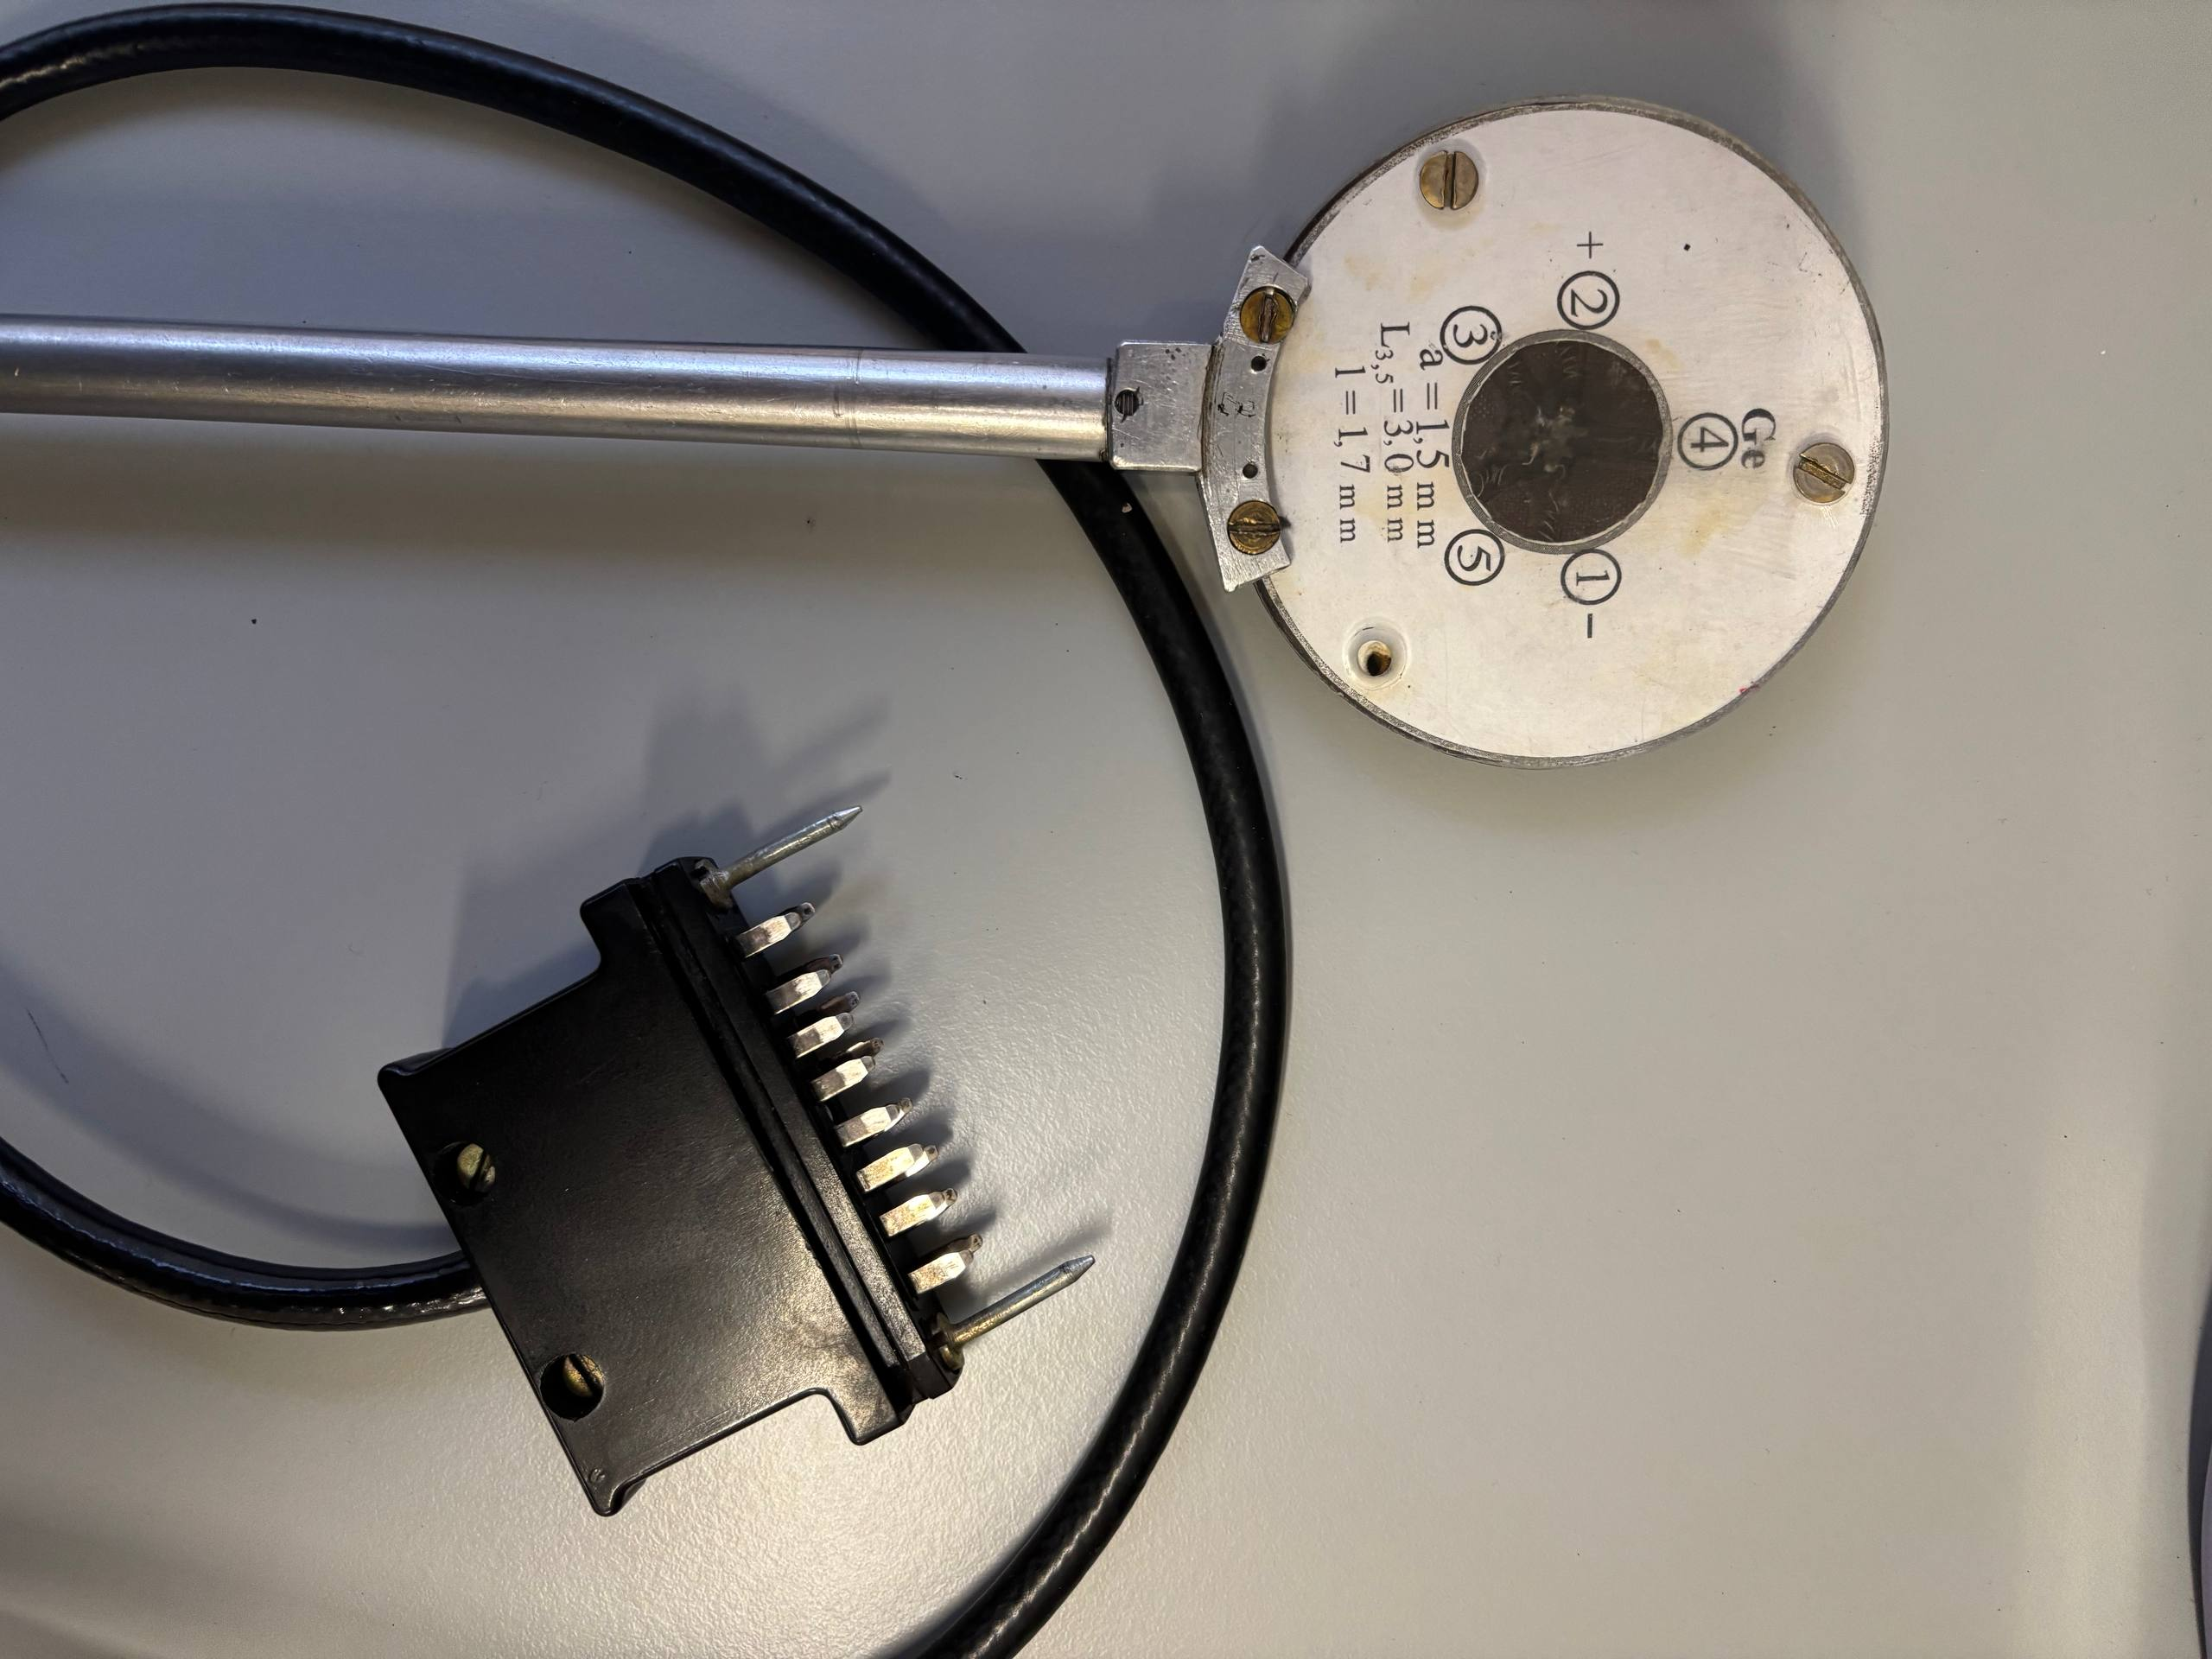
\includegraphics[height=4.6cm,angle=90,origin=c]{img/holder.jpg}\hspace{.65cm}
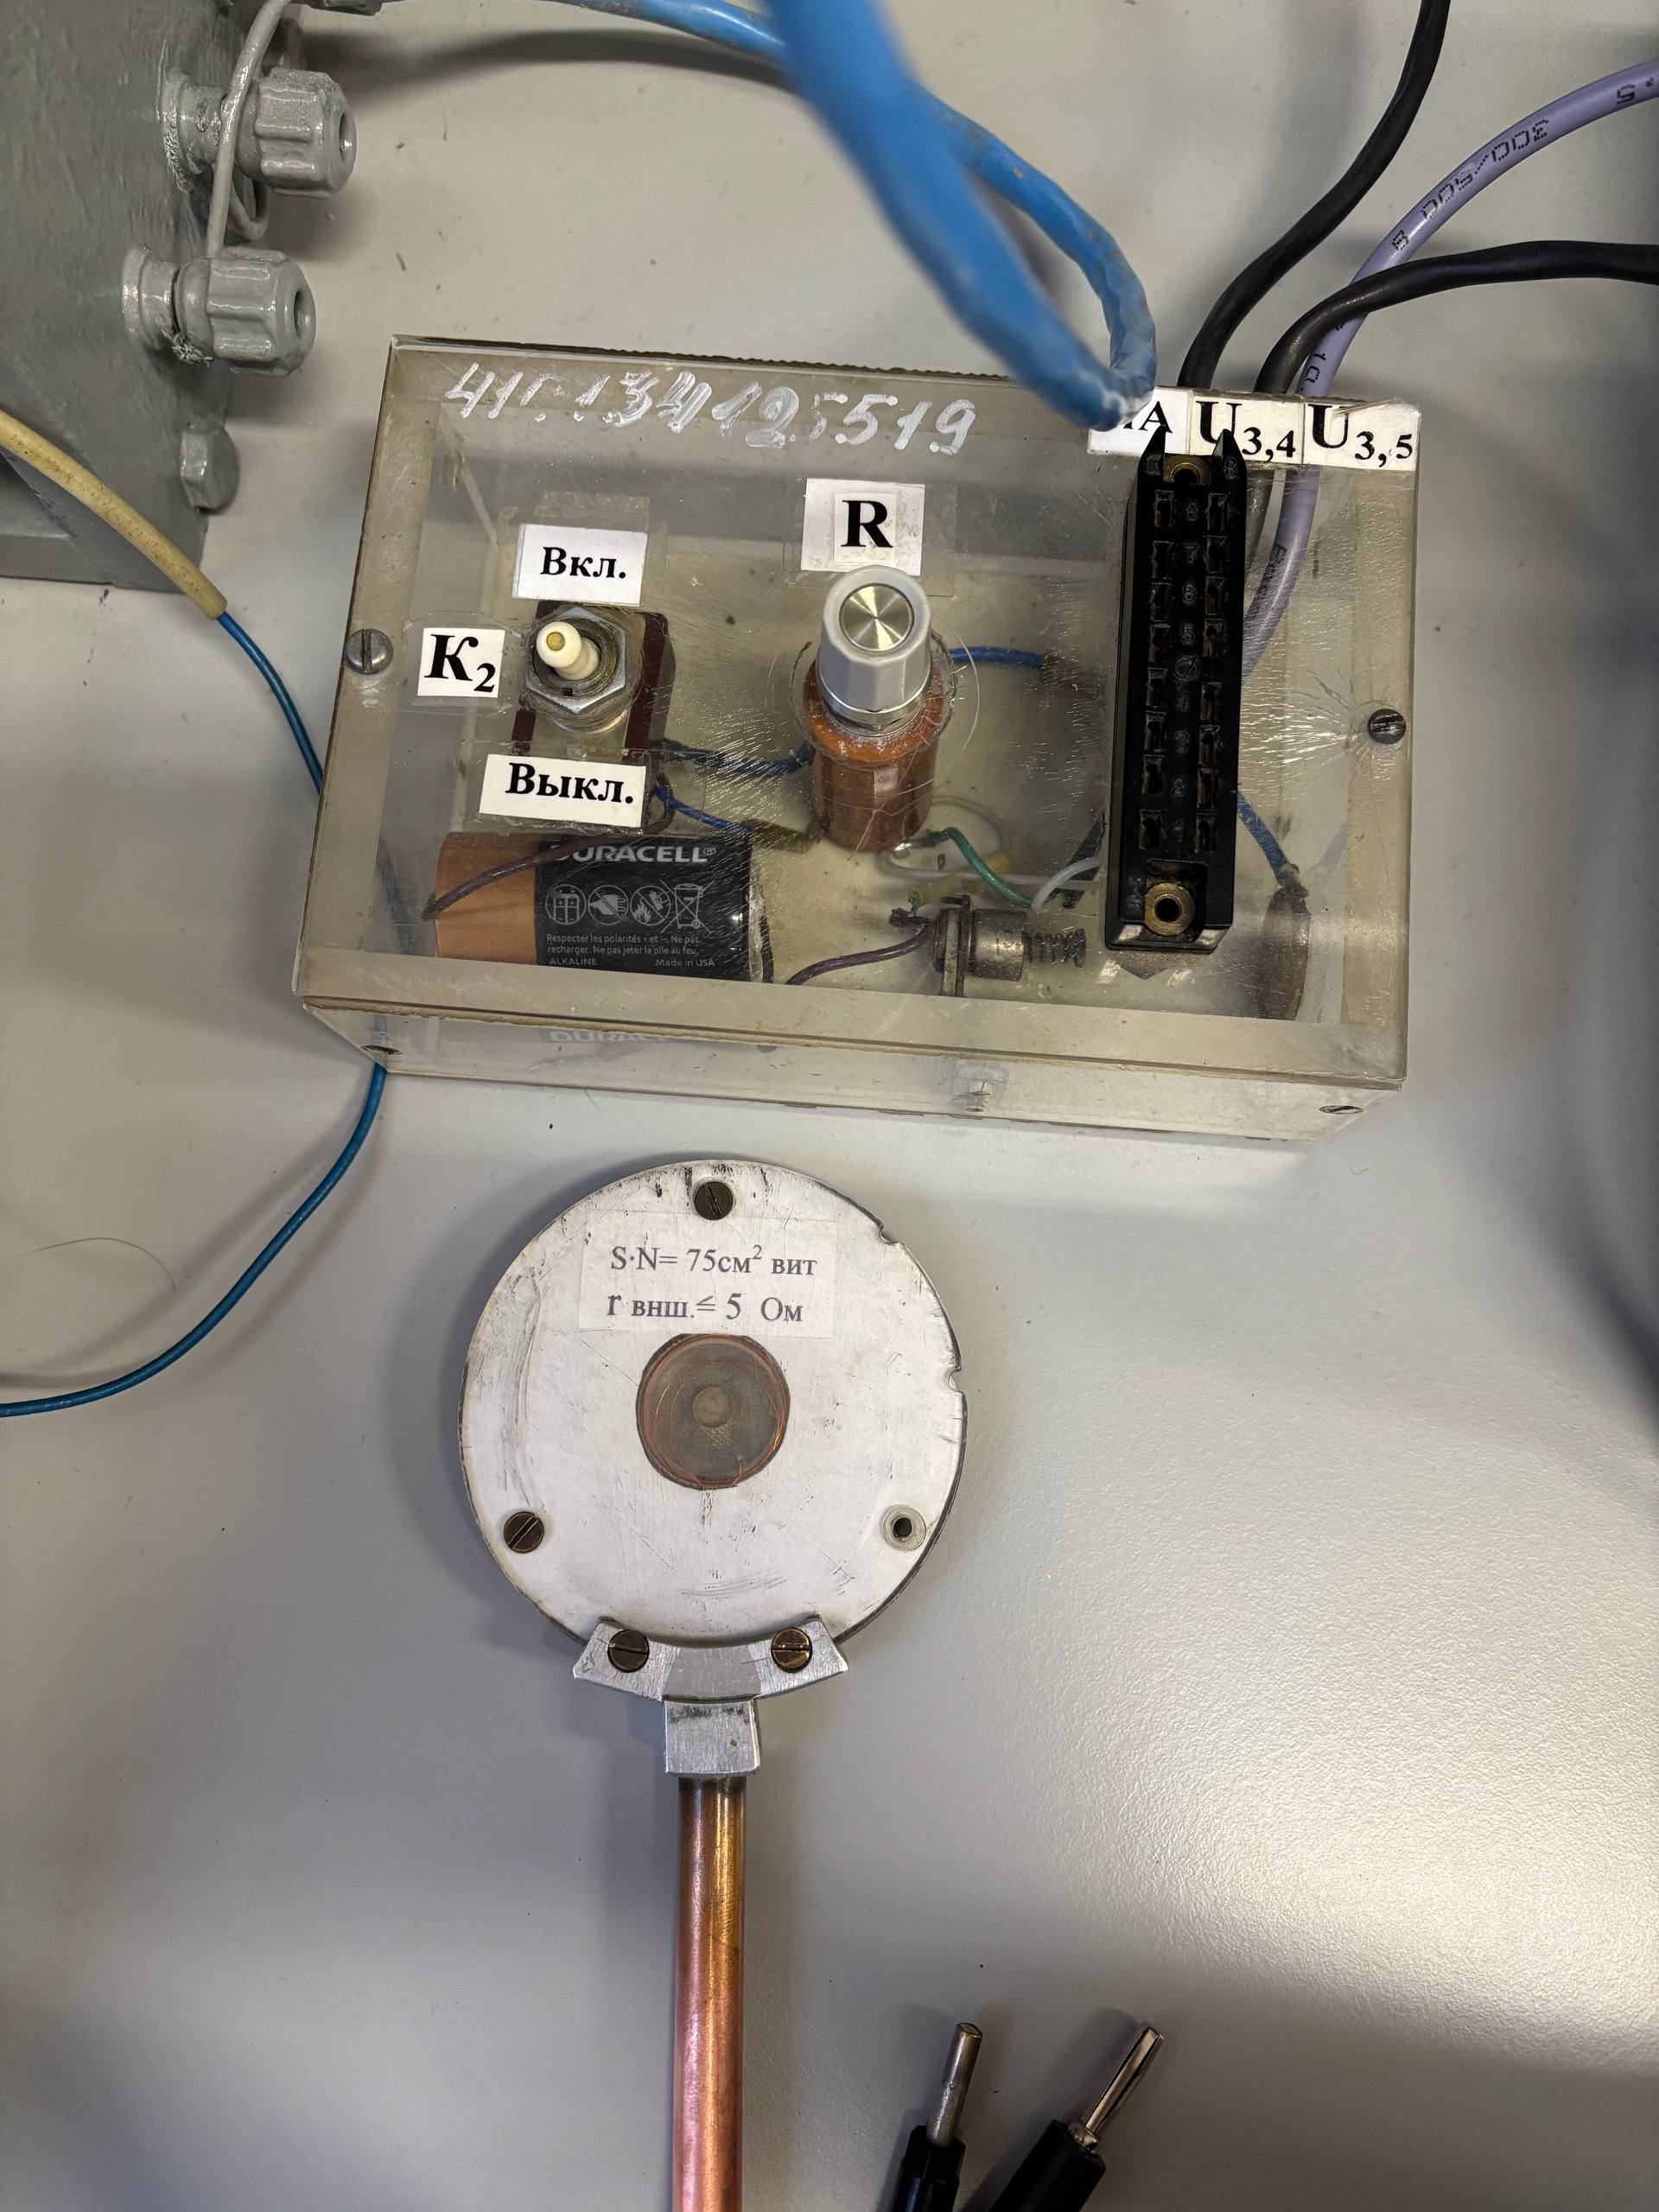
\includegraphics[height=6.1cm]{img/coil.jpg}
\caption{Слева — держатель Ge с маркировкой контактов и размерами образца. Справа — блок с ключом К2, реостатом и разъёмом, под ним пробная катушка с паспортным произведением $SN=75$~см$^2\cdot$виток и обозначением $r_{\text{внеш}}\leq5$~Ом.}\label{fig:holder}
\end{figure}
По маркировке держателя толщина $a=1{,}5$~мм, ширина $l=1{,}7$~мм, база $L_{35}=3{,}0$~мм. Ток идёт от контакта 2 ($+$) к контакту 1 ($-$). Контакты 3 и 4 расположены у противоположных краёв, 3 и 5 — вдоль одного края.

\clearpage
\section{Градуировка электромагнита}
В описании стенда от VIII-2014 предусмотрен датчик АТЕ-8702. В данном опыте градуировку выполнили милливеберметром. По инструкции от 10.08.2015 отклонение его рамки пропорционально интегралу ЭДС индукции, то есть изменению потокосцепления. Полная шкала 10~мВб содержит 10 основных делений, в журнале записаны десятые доли мВб. Для каждого тока измерение отсчитано от нуля. При вычислении $B$ каждая запись используется один раз.

\begin{table}[h!]\centering
\caption{Градуировка по пробной катушке. Поле в последнем столбце вычислено по маркировке катушки.}\label{tab:cal}
\begin{minipage}[c]{.38\linewidth}\centering\small
\begin{tabular}{ccc}\hline
$\im$, А & $|\Delta\Phi|$, мВб & $B$, Тл\\\hline
\CalibrationRows
\hline\end{tabular}
\end{minipage}\hfill
\begin{minipage}[c]{.58\linewidth}
\[
B=\frac{|\Delta\Phi|}{SN}.
\]
При $\im=1{,}62$~А получаем
\[
 \frac{8{,}9\cdot10^{-3}~\text{Вб}}{75\cdot10^{-4}~\text{м}^2}
 =1{,}187~\text{Тл}.
\]
Между узлами градуировки поле найдено линейной интерполяцией. При выключенном магните за начало отсчёта принято $B=0$. Градуировка охватывает все ненулевые токи холловских серий.
\end{minipage}
\end{table}
\begin{figure}[h!]\centering\figfile{.72}{calibration.pdf}
\caption{Индукция поля в зазоре. При увеличении тока от 0,20 до 0,40~А поле возрастает на 0,187~Тл, а от 1,30 до 1,50~А — всего на 0,067~Тл. Уменьшение наклона указывает на приближение сердечника к насыщению.}\label{fig:cal}
\end{figure}

\clearpage
\section{Поперечные измерения}
При каждом фиксированном токе образца сначала записывали $U_0$, затем $U_{34}$ при возрастающем $\im$. В серии 0,2~мА журнал ведётся в мВ, в остальных — в мкВ. Например, при 0,2~мА и $\im=0{,}15$~А получаем $U_{34}-U_0=0{,}011-(-0{,}001)=0{,}012$~мВ.
\begin{figure}[h!]\centering\figfile{.89}{hall_family.pdf}
\caption{ЭДС Холла в прямой ориентации образца. Для каждой серии показаны измерения и прямая МНК после вычитания собственного нулевого отсчёта.}\label{fig:family}
\end{figure}
\begin{table}[h!]\centering
\caption{Нули прямых серий и наклоны прямых $U_{34}-U_0=KB$.}\label{tab:slopes}
\begin{tabular}{ccc}\hline
$I$, мА & $U_0$, мкВ & $K$, мВ/Тл\\\hline
\SlopeRows
\hline\end{tabular}
\end{table}
Для прямых через начало координат $K_i=\sum_j B_j(U_{ij}-U_{0i})/\sum_j B_j^2$. Выбор начала задаётся отдельно измеренным нулём каждой серии. Аналогичная аппроксимация $K_i=s I_i$ следует из \cref{eq:hall} и даёт $s=\ResK$~В/(Тл$\cdot$А). При свободном пересечении с осью наклон составляет 0,393~В/(Тл$\cdot$А). Различие 4,7\,\% укладывается в погрешность $s$.

\clearpage
\section{Проверка обращением поля}\label{sec:rev}
\begin{figure}[h!]\centering\figfile{.64}{k_vs_I.pdf}
\caption{Наклон поперечной характеристики растёт с током образца. Наклон общей прямой определяет $|R_H|/a$.}\label{fig:ki}
\end{figure}
При $I=0{,}9$~мА для тех же семи ненулевых токов магнита измерено $U_-$ в обратной ориентации. Полуразность $D=(U_+-U_-)/2$ выделяет нечётную по полю часть. Поскольку нули серий различны, из $D$ вычтена половина их разности $D_0$. При максимальном токе магнита сырая полуразность составляет 439~мкВ.
\begin{table}[h!]\centering\small
\caption{Парные измерения при 0,9~мА. Напряжения приведены в мкВ.}
\begin{tabular}{ccccc}\hline
$\im$, А & $U_+$ & $U_-$ & $D$ & $D-D_0$\\\hline
\ReverseRows
\hline\end{tabular}
\end{table}
\begin{figure}[h!]\centering\figfile{.63}{reverse.pdf}
\caption{Проверка холловского сигнала при смене направления поля относительно образца.}\label{fig:rev}
\end{figure}

\clearpage
\section{Продольное измерение и погрешности}
При $I=0{,}9$~мА без поля $U_{35}$ изменилось от $-1{,}570$ до $-1{,}580$~мВ. Во второй записи над зачёркнутыми цифрами вписано «80». Модуль среднего равен 1,575~мВ, половина размаха 0,005~мВ учтена как вклад дрейфа. Сопротивление участка $R_{35}=1{,}575/0{,}9=1{,}75$~Ом. Прямая подстановка в \cref{eq:long} даёт
\[
 \sigma=\frac{0{,}0009\cdot0{,}0030}
 {0{,}001575\cdot0{,}0015\cdot0{,}0017}=672{,}3~\text{См/м}.
\]

При отсутствии паспортного класса шкале каждого прибора приписана общая относительная погрешность 3\,\%. Отдельно учтена единица последнего разряда записи: 0,1~мВб для потокосцепления, 0,01~А для тока магнита, 0,1~мА для тока образца и 1~мкВ для напряжений. Для размеров с держателя приняты допуски по 0,1~мм, для $SN$ — 1~см$^2\cdot$виток. Эти оценки основаны на точности записи. Фактические допуски маркировки неизвестны.

Погрешности перенесены через обе регрессии по частным производным. Независимые вклады сложены в квадратуре вместе со стандартными ошибками наклонов по остаткам. Один и тот же $U_0$ смещает все точки одной серии, а узел градуировки влияет сразу на все точки, интерполированные с его участием. Такие входы варьировались совместно. Для $|R_H|$ существенны погрешность наклона $s$ (8,1\,\%) и толщины (6,7\,\%). В проводимости заметен вклад разряда тока $0{,}1/0{,}9=11\,\%$.

В произведении $\mu_H=\sigma|R_H|=|s| I L_{35}/(|U_{35}|l)$ толщина сокращается. Тот же масштаб миллиамперметра входит в $I$ и в знаменатель наклона $s$; общий масштаб вольтметра входит в $s$ и $U_{35}$. При расчёте погрешности подвижности эти корреляции учтены.

\section{Обсуждение и заключение}
\begin{table}[h!]\centering
\caption{Электрические характеристики образца Ge. Погрешности рассчитаны по принятым для установки оценкам.}\label{tab:results}
\begin{tabular}{lcc}\hline
Величина и единица & Результат & Отн. погрешность\\\hline
$|R_H|$, м$^3$/Кл & $\ResRHabs$ & $\RelRH\,\%$\\
$n_H$, м$^{-3}$ & $\ResN$ & $\RelN\,\%$\\
$\rho$, Ом$\cdot$м & $\ResRho$ & $\RelRho\,\%$\\
$\sigma$, См/м & $\ResSigma$ & $\RelSigma\,\%$\\
$\mu_H$, м$^2$/(В$\cdot$с) & $\ResMuSI$ & $\RelMu\,\%$\\
$\mu_H$, см$^2$/(В$\cdot$с) & $\ResMu$ & $\RelMu\,\%$\\\hline
\end{tabular}
\end{table}

\clearpage
\subsection*{Что показывает обращение поля}
При наибольшем общем токе магнита, 1,54~А, получено $D-D_0=430{,}5$~мкВ, а по прямому измерению $400-(-29)=429$~мкВ. Наклон по семи парным точкам $\ResKrev$~мВ/Тл совпадает в пределах погрешности с прямым наклоном $0{,}374\pm0{,}017$~мВ/Тл. Общие градуировка и прямая серия входят в оба расчёта. Согласие свидетельствует о нечётности поперечного сигнала по полю.

В прямой серии при 0,9~мА исправленный нуль прочитан как $-29$~мкВ. Если последняя цифра означает 2, получаются $K=0{,}366$ вместо $0{,}374$~мВ/Тл и уменьшение итогового $|R_H|$ на 0,61\,\%. В обратной серии под зачёркнутой цифрой вписана 6, то есть $U_0=-46$~мкВ. Это объясняет поправку $D_0=8{,}5$~мкВ. Последний отсчёт серии 0,3~мА принят за 150~мкВ. При чтении 180~мкВ $|R_H|$ увеличился бы на 0,16\,\%. Обе неоднозначности меньше погрешности результата. Все точки сохранены.

\subsection*{Знак носителей}
Полярность держателя определяет направление обычного тока $2\to1$. Вольтметр показывает потенциал входа «U» относительно «0». При подключении $3\to\text{«U»}$, $4\to\text{«0»}$ положительное приращение означает рост потенциала контакта 3 относительно 4. Методика задаёт эту схему, но фактические подключения входов при записи серии на фото не прослеживаются. Стрелка на магните обозначает направление тока в обмотке при положении I разъёма К1. В журнале не зафиксировано, какой стороной к соответствующему полюсу стоял держатель в прямой серии. Поэтому восстановить направление $\mathbf j\times\mathbf B$ относительно контактов и присвоить знак $R_H$ по этим материалам нельзя.

\subsection*{Сопоставление со свойствами германия}
Для собственного Ge при 300~К справочник ФТИ [3] даёт $n_i=2{,}0\cdot10^{13}$~см$^{-3}$ и $\rho_i=46$~Ом$\cdot$см. Здесь $n_H=\ResNcm$~см$^{-3}$, примерно в 500 раз выше, а $\rho\simeq0{,}149$~Ом$\cdot$см примерно в 310 раз ниже. Обе величины согласуются с тем, что образец легирован.

Справочные ориентиры подвижности электронов и дырок при комнатной температуре составляют 3900 и 1900~см$^2$/(В$\cdot$с) соответственно [4]. Для слабо компенсированного $n$-Ge при $N_D\simeq10^{16}$~см$^{-3}$ эмпирическая формула Хилсума даёт $3900/\sqrt{1+10^{-17}N_D}\simeq3720$~см$^2$/(В$\cdot$с). Измеренная $\mu_H=\ResMu$~см$^2$/(В$\cdot$с) ближе к электронному ориентиру и согласуется с этой оценкой в пределах погрешности. Сопоставление предполагает комнатную температуру: вид и концентрация примеси, степень компенсации и температура образца отдельно не измерялись. Знак заряда определяется ориентационным опытом. При $T=300$~К и единичном холл-факторе соотношение Эйнштейна даёт $D=\mu_H k_BT/e\simeq108$~см$^2$/с. Оценка частоты столкновений $\nu=e/(m^*\mu_H)$ и длины пробега $\lambda=\sqrt{3k_BT/m^*}/\nu$ дополнительно требует эффективной массы для конкретного типа носителей.

\clearpage
\section*{Приложение. Первичные поперечные измерения}
В каждой паре столбцов верхний заголовок задаёт ток образца $I$, первый столбец — ток магнита $\im$ в амперах, второй — показание $U_{34}$. Нули указаны в \cref{tab:slopes}, обратная серия приведена в разделе~\ref{sec:rev}.
\begin{center}\small
\begin{tabular}{cccccccc}\hline
\multicolumn{2}{c}{$0{,}2$ мА} & \multicolumn{2}{c}{$0{,}3$ мА} & \multicolumn{2}{c}{$0{,}4$ мА} & \multicolumn{2}{c}{$0{,}5$ мА}\\
$I_{\mathrm M}$, А & $U_{34}$, мВ & $I_{\mathrm M}$, А & $U_{34}$, мкВ & $I_{\mathrm M}$, А & $U_{34}$, мкВ & $I_{\mathrm M}$, А & $U_{34}$, мкВ\\\hline
$0{,}15$ & $+0{,}011$ & $0{,}20$ & $20$ & $0{,}20$ & $26$ & $0{,}20$ & $30$\\
$0{,}30$ & $+0{,}025$ & $0{,}40$ & $47$ & $0{,}40$ & $59$ & $0{,}43$ & $80$\\
$0{,}46$ & $+0{,}040$ & $0{,}60$ & $73$ & $0{,}61$ & $94$ & $0{,}58$ & $110$\\
$0{,}62$ & $+0{,}055$ & $0{,}80$ & $97$ & $0{,}80$ & $125$ & $0{,}80$ & $151$\\
$0{,}75$ & $+0{,}067$ & $1{,}00$ & $118$ & $0{,}99$ & $150$ & $1{,}05$ & $192$\\
$0{,}90$ & $+0{,}078$ & $1{,}20$ & $133$ & $1{,}19$ & $169$ & $1{,}28$ & $215$\\
$1{,}05$ & $+0{,}088$ & $1{,}40$ & $143$ & $1{,}39$ & $183$ & $1{,}54$ & $233$\\
$1{,}20$ & $+0{,}096$ & $1{,}57$ & $150$ & $1{,}55$ & $192$ &  & \\
$1{,}35$ & $+0{,}101$ &  &  &  &  &  & \\
$1{,}50$ & $+0{,}106$ &  &  &  &  &  & \\
\hline\end{tabular}
\end{center}
\begin{center}\small
\begin{tabular}{cccccccc}\hline
\multicolumn{2}{c}{$0{,}6$ мА} & \multicolumn{2}{c}{$0{,}7$ мА} & \multicolumn{2}{c}{$0{,}8$ мА} & \multicolumn{2}{c}{$0{,}9$ мА}\\
$I_{\mathrm M}$, А & $U_{34}$, мкВ & $I_{\mathrm M}$, А & $U_{34}$, мкВ & $I_{\mathrm M}$, А & $U_{34}$, мкВ & $I_{\mathrm M}$, А & $U_{34}$, мкВ\\\hline
$0{,}21$ & $37$ & $0{,}20$ & $39$ & $0{,}20$ & $45$ & $0{,}24$ & $65$\\
$0{,}42$ & $91$ & $0{,}41$ & $100$ & $0{,}40$ & $109$ & $0{,}40$ & $123$\\
$0{,}59$ & $131$ & $0{,}60$ & $153$ & $0{,}59$ & $172$ & $0{,}60$ & $192$\\
$0{,}80$ & $178$ & $0{,}80$ & $205$ & $0{,}83$ & $241$ & $0{,}79$ & $255$\\
$1{,}00$ & $217$ & $1{,}01$ & $252$ & $1{,}09$ & $302$ & $1{,}07$ & $331$\\
$1{,}26$ & $251$ & $1{,}23$ & $286$ & $1{,}37$ & $342$ & $1{,}28$ & $369$\\
$1{,}53$ & $274$ & $1{,}54$ & $316$ & $1{,}54$ & $359$ & $1{,}54$ & $400$\\
\hline\end{tabular}
\end{center}


\section*{Источники}
\raggedright
\begin{enumerate}
\item МФТИ. Эффект Холла в полупроводниках. Работа 3.3.4 (4.11Б-2). Дополнительное описание, редакция VIII-2014.
\item Милливеберметр. Устройство и принцип действия. Правила работы. Инструкция к стенду, 10 августа 2015~г.
\item ФТИ им. А.\,Ф.~Иоффе. NSM Archive. Germanium. Band structure and carrier concentration.\par{\small\url{https://www.ioffe.ru/SVA/NSM/Semicond/Ge/bandstr.html}}
\item ФТИ им. А.\,Ф.~Иоффе. NSM Archive. Germanium. Electrical properties, раздел Mobility and Hall Effect.\par{\small\url{https://www.ioffe.ru/SVA/NSM/Semicond/Ge/electric.html}}
\end{enumerate}
\end{document}
